\documentclass[10pt]{beamer}

\mode<presentation> 
{ \usetheme[nat,dogma]{Frederiksberg} }

% \usepackage[danish]{babel}
\usepackage[latin1]{inputenc}
\usepackage{times}
\usepackage[T1]{fontenc}
\usepackage[english]{babel}
\usepackage{hyperref}

\usepackage{multimedia}
\usepackage{francois-preamble}
\usepackage{multirow}

% \usepackage{multimedia}


\newcommand{\cc}{{c\!\!,}}
\newcommand{\degr}[1]{{{#1}^\circ}}

\title{Segmentation -- Snake, Discrete Formulation and Algorithm (almost) without the
  Painfully Agonizing Details}

\author[F.~Lauze] % (optional, use only with lots of authors)
{Fran{\c c}ois Lauze}

\institute[DIKU] % (optional, but mostly needed)
{
  Department of Computer Science\\
  University of Copenhagen
}

\date[2012 B2] % (optional, should be abbreviation of conference name)
% {Research Presentation, Diku 2006}

\definecolor{gold}{rgb}{0.95,0.83,0.0}
\definecolor{orange}{rgb}{0.95,0.7,0.0}
% \definecolor{backblue}{rgb}{0.93,0.94,0.99}
\definecolor{backblue}{rgb}{0.95,0.94,0.99}
\setbeamercolor*{background canvas}{bg=backblue} 



\newcommand{\myemph}[1]{{\color{blue}{#1}}}
\newcommand{\intrg}[1]{\int_{{#1}=-\infty}^\infty}
\newcommand{\intRR}{\int_{-\infty}^\infty}

\AtBeginSection[]
{
  \begin{frame}<beamer>{Outline}
    \tableofcontents[currentsection,currentsubsection]
  \end{frame}
}

\begin{document}
\maketitle

% would be cool with more images showing applications


%-------------------------------------------------------------------
%   Start slides
%-------------------------------------------------------------------




%----------------------------------------------

\begin{frame}
  \frametitle{Discrete Formulation}
  \begin{itemize}
  \item In the sequel, subtracting two points in the plane means getting the vectors joining them, and means subtracting
    their coordinates
    $$
    P_1 = (4,3),\quad P_2 = (1,2),\quad P_2-P_1 = \overrightarrow{P_1P_2} = (-3,-1). 
    $$
    \begin{center}
      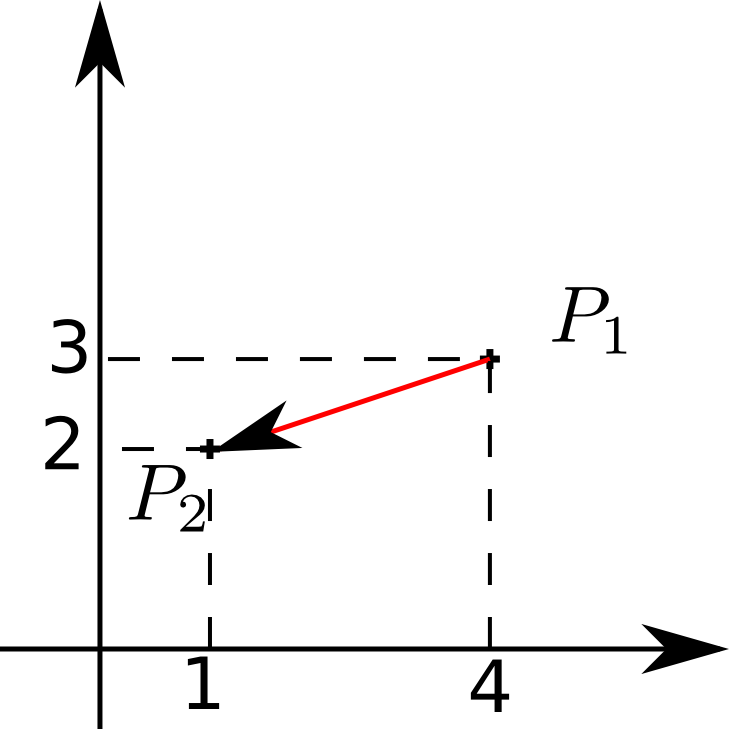
\includegraphics[width=0.35\textwidth]{FIGURES/diffpoints}
    \end{center}
  \item The length of vector $P_2-P_1$ is denoted $\|P_2-P_1\|$ and is $\sqrt{(x_2-x_1)^2 + (y_2-y_1)^2}$.
  \end{itemize}
\end{frame}


\begin{frame}
  \frametitle{Curve representation}
  \begin{itemize}
  \item A closed curve $C$ will be represented by $n$ points $P_1,P_2,\dots,P_n$, and consecutive points are joined
    by line segments, and with $P_{n+1} = P_1,$, $P_0=P_n$ indicating that the curve is closed: 
    \begin{center}
      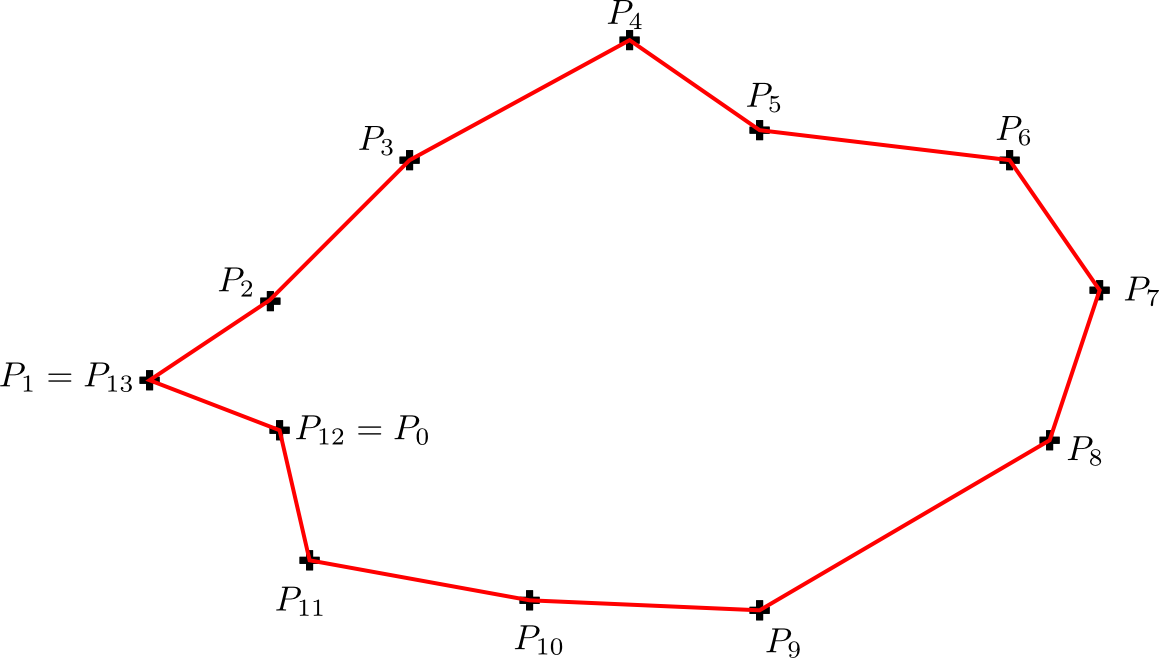
\includegraphics[width=0.75\textwidth]{FIGURES/closedcurvepoints}\\
      A closed curve with 12 points
    \end{center}
  \end{itemize}
\end{frame}


\begin{frame}
  \frametitle{Discrete Snake Energy: Curve Internal Forces}
  \begin{itemize}
  \item Curve Energy term: sum of squared length of the curve segments:
    $$
    E_\Cc(C) = \sum_{i=1}^n\|P_{i+1}-P_i\|^2,\quad P_{n+1} = P_1.
    $$
  \item Bending energy term: sum squared-length of  differences of consecutive segments
    \begin{align*}
      E_\Bb(C) &= \sum_{i=1}^n\| (P_{i+1}-P_i) - (P_i-P_{i-1})\|^2\\
      &=\sum_{i=1}^n\| P_{i+1}-2P_i+P_{i-1}\|^2,\quad P_{n+1} = P_1, P_0 = P_n.
    \end{align*}
  \end{itemize}
\end{frame}


\begin{frame}
   \frametitle{Discrete Snake Energy: External (Image) Forces}
   \begin{itemize}
   \item
     $F$ is an image derived from the image $I$ to be segmented, with the property that
     $F$ should be small when at an edge of $I$ and large when at a flat region of $I$. 
   \item Standard example is 
     $$
     F = -\|\nabla I_\sigma\|^2 = -\left(I_{\sigma x}^2 + I_{\sigma y}^2\right)^2.
     $$
     with $I_\sigma = g_\sigma\ast I$, $I$ convolved with Gaussian of standard deviation $\sigma$.
   \item External force at point $P = (x,y)$: $F(P) = F(x,y)$ and external / image energy:
     $$
     E_\Ee(C) = \sum_{i=1}^n F(P_i).
     $$
   \end{itemize}
 \end{frame}



 \begin{frame}
   \frametitle{External Forces: Example}
   \begin{itemize}
   \item Using the force term $F= -\|\nabla I_\sigma\|^2$, dark indicates edge:
     \begin{center}
       \begin{tabular}[h]{cc}
          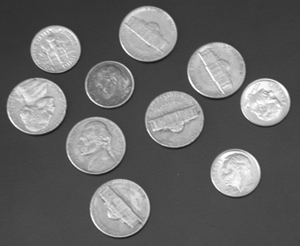
\includegraphics[width=0.45\textwidth]{IMAGES/coins} & 
          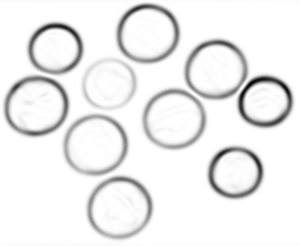
\includegraphics[width=0.45\textwidth]{IMAGES/cannyextcoins} \\
          Original image & Force term with $\sigma = 3$
       \end{tabular}
     \end{center}
   \end{itemize}
 \end{frame}

 \begin{frame}
   \frametitle{Snake Energy}
   \begin{itemize}
   \item Given a discrete closed curve $C = (P_1,P_2,\dots,P_n)$, its Snake Energy is 
     \begin{align*}
       E_\Ss(C) &= \alpha E_\Cc(C) + \beta E_\Bb(C) + \gamma E_\Ee(C)\\
       &= \alpha\sum_{i=1}^n\|P_{i+1}\!-P_i\|^2 \!\!+ \beta\sum_{i=1}^n\|P_{i+1}\!-2P_i+p_{i-1}\|^2 \!\!+ \gamma\sum_{i=1}^n F(P_i)\\
       &=\sum_{i=1}^n\left(\alpha\|P_{i+1}-P_i\|^2+\beta\|P_{i+1}-2P_i+P_{i-1}\|^2+\gamma F(P_i)\right).
     \end{align*}
   \item $\alpha$, $\beta$ and $\gamma$ are 3 weights (i.e., positive numbers) that
     provide the trade-off between the different parts.
   \end{itemize}
 \end{frame}


 \begin{frame}
  \frametitle{Solving the segmentation}
  {\small
    \begin{itemize}
     \item This is done iteratively by moving the current estimate $C^s = (P_1^s =
       (x_1^2,y_1^s), P_2^s = (x_2^2,y_2^s),\dots, P_n^n = (x_n^s,y_n^s))$ of the contour to
       the next one $C^{s+1} = (P_1^{s+1},P_2^{s+1},\dots,P_n^{s+1})$ in such a way that the
       snake energy decreases most.  This needs small steps.
     \item The theory shows that a solution can be described as solution of the systems of
       linear equations
     \end{itemize}
   }
   \begin{columns}
     \column{0.47\textwidth}
     {\small $$ M 
       \begin{pmatrix}
         x^{s+1}_1\\x^{s+1}_2\\\vdots\\x^{n+1}_N
       \end{pmatrix}
       = \begin{pmatrix}
         x^{s}_1 - \gamma F_x(x_1^{s},y_1^{s})\\
         x^{s}_2 - \gamma F_x(x_2^{s},y_2^{s})\\
         \vdots\\
         x^{s}_n - \gamma F_x(x_n^{s},y_n^{s})\\
       \end{pmatrix}
       $$}
     \column{0.47\textwidth} 
     {\small $$ M 
       \begin{pmatrix}
         y^{s+1}_1\\y^{s+1}_2\\\vdots\\y^{s+1}_N
       \end{pmatrix}
       = \begin{pmatrix}
         y^{s}_1 - \gamma F_y(x_1^{s},y_1^{s})\\
         y^{s}_2 - \gamma F_y(x_2^{s},y_2^{s})\\
         \vdots\\
         y^{s}_n - \gamma F_y(x_n^{s},y_n^{s})\\
       \end{pmatrix}
       $$}
   \end{columns}
   {\small
     \begin{itemize}
     \item $F_x$ and $F_y$ are the $x-$ and $y-$derivatives of the external force $F$, described later
     \item $M$ is the system matrix (coefficients of the systems of equations) described
       in an example in the slide next to the following one.
     \end{itemize}
   }
 \end{frame}
 
 \begin{frame}
   \begin{itemize}
   \item Solving the system of equations of the previous slide means to compute the new
     values $x_i^{s+1}$ and $y_i^{s+1}$ as follows:
   \end{itemize}
   \begin{columns}
     \column{0.47\textwidth}
     {\small $$
       \begin{pmatrix}
         x^{s+1}_1\\x^{s+1}_2\\\vdots\\x^{n+1}_N
       \end{pmatrix}
       = M ^{-1} \begin{pmatrix}
         x^{s}_1 - \gamma F_x(x_1^{s},y_1^{s})\\
         x^{s}_2 - \gamma F_x(x_2^{s},y_2^{s})\\
         \vdots\\
         x^{s}_n - \gamma F_x(x_n^{s},y_n^{s})\\
       \end{pmatrix},
       $$}
     \column{0.47\textwidth} 
     {\small $$ 
       \begin{pmatrix}
         y^{s+1}_1\\y^{s+1}_2\\\vdots\\y^{s+1}_N
       \end{pmatrix}
       = M^{-1} \begin{pmatrix}
         y^{s}_1 - \gamma F_y(x_1^{s},y_1^{s})\\
         y^{s}_2 - \gamma F_y(x_2^{s},y_2^{s})\\
         \vdots\\
         y^{s}_n - \gamma F_y(x_n^{s},y_n^{s})\\
       \end{pmatrix}
       $$}
   \end{columns}
   \begin{itemize}
   \item $M^{-1}$ is the \myemph{inverse matrix} of $M$.
   \item This is the same matrix for both the abscissas and ordinates.
   \end{itemize}
 \end{frame}


 \begin{frame}
   \frametitle{System Matrix}
   \begin{itemize}
   \item Set $A = \tau\beta$, $B = -\tau(\alpha + 4\beta)$, $C = 1+ \tau(2\alpha + 6\beta)$,
   \item   Here is the matrix of the linear system for a curve represented by  10 points.
     {\small $$ M = 
       \begin{pmatrix}
         C & B & A & 0 & 0 & 0 & 0 & 0 & A & B \\
         B & C & B & A & 0 & 0 & 0 & 0 & 0 & A \\
         A & B & C & B & A & 0 & 0 & 0 & 0 & 0 \\
         0 & A & B & C & B & A & 0 & 0 & 0 & 0 \\
         0 & 0 & A & B & C & B & A & 0 & 0 & 0 \\
         0 & 0 & 0 & A & B & C & B & A & 0 & 0 \\
         0 & 0 & 0 & 0 & A & B & C & B & A & 0 \\
         0 & 0 & 0 & 0 & 0 & A & B & C & B & A \\
         A & 0 & 0 & 0 & 0 & 0 & A & B & C & B \\
         B & A & 0 & 0 & 0 & 0 & 0 & A & B & C \\
       \end{pmatrix}
       $$}
   \item
     Note the values at the upper-right and lower down corners. This is
     because we deal with closed curves.
   \end{itemize}
 \end{frame}
 
 
 \begin{frame}
   \frametitle{System Matrix II}
   \begin{itemize}
   \item Constructing the system matrix is easy. Python possesses a \texttt{roll()} function
     in \texttt{numpy} that rolls and wraps the content of a vector. 
   \item Each line can be obtained from the previous by proper rolling! Easy!
   \item Matlab has a command called \texttt{toeplitz()} that can construct the system matrix
     very easily.
   \item When the system matrix has been computed, it can be immediately
     \myemph{inverted}. \texttt{numpy.linagl.inv()} does the job for python, while \texttt{inv()} will do it for Matlab.
   \end{itemize}
 \end{frame}


 \begin{frame}
   \frametitle{Derivatives of external forces}
   An example using the one described before.
   \begin{center}
     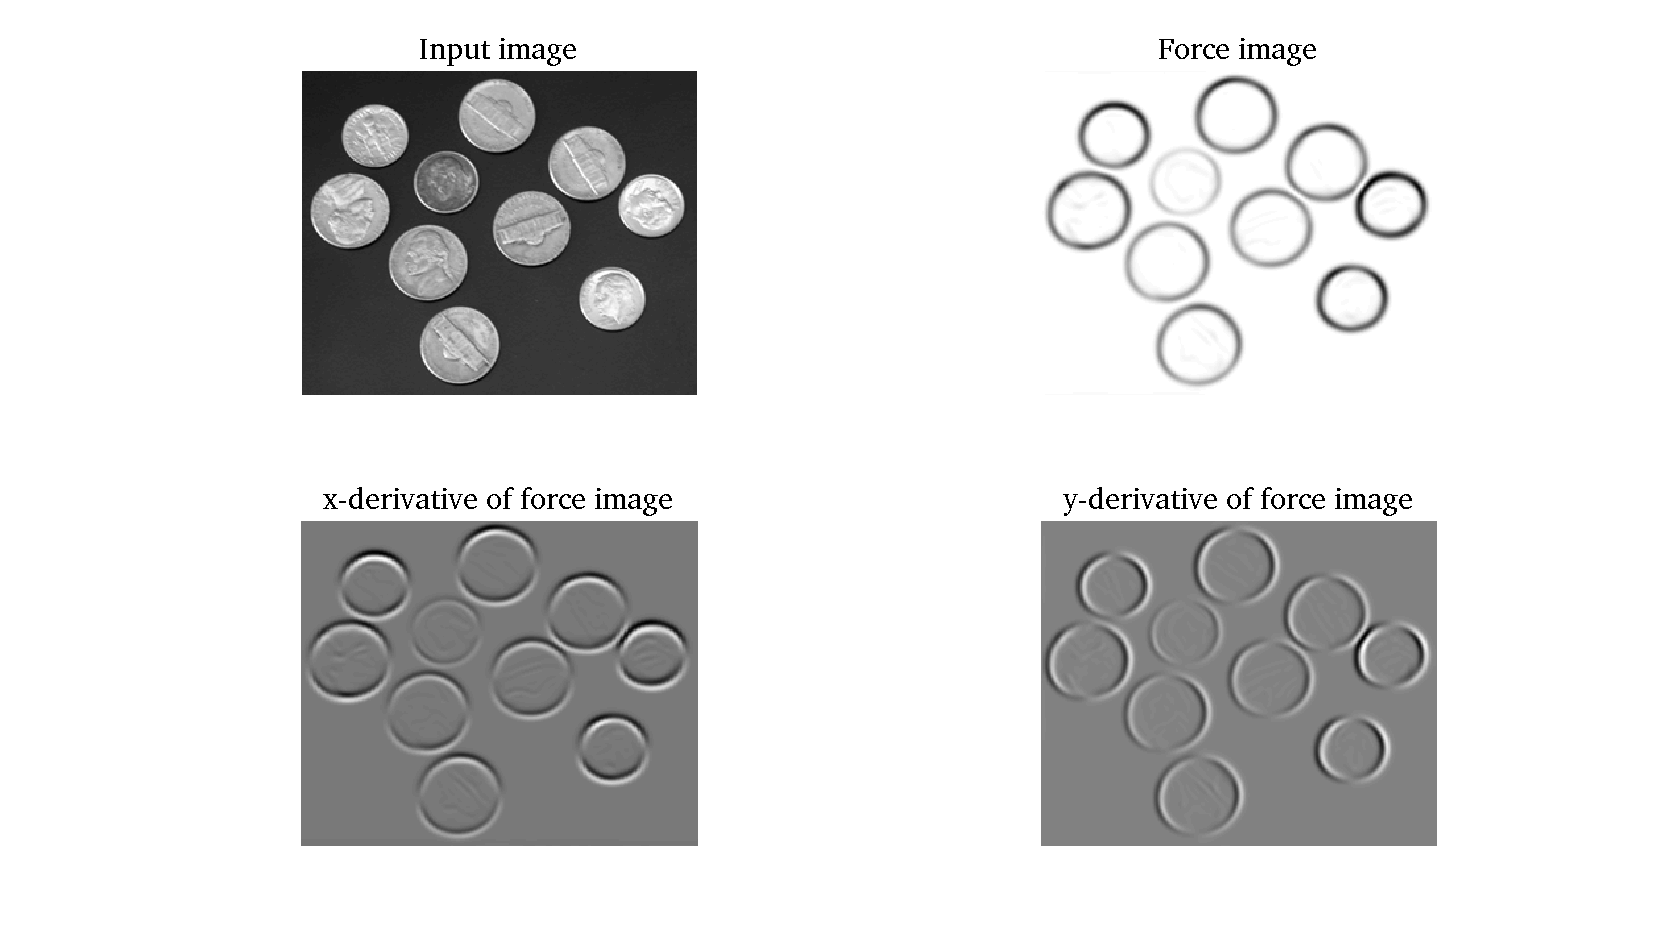
\includegraphics[width=1\textwidth]{FIGURES/externforces}
   \end{center}
 \end{frame}

 \begin{frame}
   {\small
   \begin{itemize}
   \item A direct calculation shows that for $F = -\|\nabla I_\sigma\|^2$, 
     $$
     F_x = -2\left(I_{\sigma x}I_{\sigma xx} + I_{\sigma y}I_{\sigma xy}\right),\quad 
     F_y = -2\left(I_{\sigma x}I_{\sigma xy} + I_{\sigma y}I_{\sigma yy}\right).
     $$
   \item Main difficulty in computing $F_x$ (or $F_y$) at $(x,y)$: values
     of $F_x$  generally only known at grid position $(i,j)$, $i=0\dots M-1$, $j=0\dots
     N-1$ with $M\times N$ size of image $I$ (and also of $F$, $F_x$ and $F_y$). But
     $(x,y)$ might not be on the grid. Need for interpolation.
   %\end{itemize}
   %\vspace{-4mm}
   \begin{columns}
     \column{0.45\textwidth}
     \begin{center}
       \includegraphics[width=0.9\textwidth]{FIGURES/bilininterp}\\
       Bilinear Interpolation
     \end{center}
     \column{0.45\textwidth}
     \begin{align*}
       F(x,y)&\approx F(i,j)(1-h_i)(1-h_j)\\ 
       &+ F(i+1,j)h_i(1-h_j)\\
       &+ F(i,j+1)(1-h_i)h_j\\
       &+ F(i+1.j+1)h_i h_j
     \end{align*}
   \end{columns}
   %\begin{itemize}
   \item A good choice: bilinear or bicubic interpolation. Matlab built-in function
     \texttt{interp2} does it.  I have provided a Python class to do it.
 \end{itemize}
 }
\end{frame}


\begin{frame}
  \frametitle{Wrap-up: Algorithm Sketch}
  \begin{enumerate}
  \item Input image $I$. Weights $\alpha$, $\beta$, $\gamma$ given. Time step $\tau$ given.
  \item Select the number $n$ of points and the initial points $P_1^0 = (x_1^0,y_1^0)$, 
    $P_2^0 = (x_2^0,y_2^0)$, \dots ,$P_n^0 = (x_n^0,y_n^0)$  
  \item Compute the system matrix $M = M(\alpha,\beta,\tau)$ of size $n\times n$ and its
    inverse $Q = M^{-1}$.
  \item Compute derivatives $F_x$ and $F_y$ of external force image $F$
  \item Iterate until convergence (or 42 iterations for instance, \`a la HHGTTG)
    \begin{columns}
      \column{0.4\textwidth} 
      {\small $$
        \begin{pmatrix}
          x^{s+1}_1\\x^{s+1}_2\\\vdots\\x^{n+1}_N
        \end{pmatrix} = 
        Q \begin{pmatrix}
          x^{s}_1 - \gamma F_x(x_1^{s},y_1^{s})\\
          x^{s}_2 - \gamma F_x(x_2^{s},y_2^{s})\\
          \vdots\\
          x^{s}_n - \gamma F_x(x_n^{s},y_n^{s})\\
        \end{pmatrix},
        $$}
      \column{0.4\textwidth}  {\small $$ 
        \begin{pmatrix}
          y^{s+1}_1\\y^{s+1}_2\\\vdots\\y^{s+1}_N
        \end{pmatrix}
        = Q \begin{pmatrix}
          y^{s}_1 - \gamma F_y(x_1^{s},y_1^{s})\\
          y^{s}_2 - \gamma F_y(x_2^{s},y_2^{s})\\
          \vdots\\
          y^{s}_n - \gamma F_y(x_n^{s},y_n^{s})\\
        \end{pmatrix}
        $$}
    \end{columns}
    The values $F_x(x_i^s,y_i^s)$ and $F_y(x_i^s,y_i^s)$ being interpolated from the
    derivative external force images.
  \end{enumerate}
\end{frame}

\begin{frame}
  \frametitle{Interactivity...}
  \begin{itemize}
  \item I have said nothing about point selection, plotting and interactivity (up to some level).
  \item Up to the implementers to decide.
  \item One must be careful that selected points with figures and mouse are in general in
    a different coordinate system than the usual image / array indexing / coordinates
    system.
  \item That's all folks!
  \end{itemize}
\end{frame}


\end{document}

